
\section{Motivation}

The rapid growth of data generated and collected in large-scale information systems leads to new opportunities for  society and businesses. 
By the end of 2020, the total amount of generated data is estimated to be 44 trillion gigabytes of which 90\% has been created in the last two years \cite{datagrowth}.
In order to benefit from the massive amount of data, efficient solutions are required, that are able to extract potential value in form of models, insights and predictions.

A remarkable subset of this data can be described as \textit{event data}, which is generated by \textit{process-aware information systems}, which define, manage and execute business processes \cite{DBLP:journals/topnoc/Aalst09}.
With the non stopping rise of digitization of business processes, increasingly more event data becomes utilizable, thus the potential value of this data is rising sharply.

The scientific engagement aiming to discover, analyze and improve real processes based on event data led to \textit{process mining}. Process mining bridges the gab between the data-driven characteristic of data science and the process-centric view of process science \cite{DBLP:books/sp/Aalst16}.
The ongoing success of progress mining in research has been transferred to businesses, that successfully offer or utilize this technology.
Celonis, which is often considered as one of the biggest commercial providers of process mining, has been valued 2.5 billion dollar only 9 years after the company was founded \cite{celonis}.

Modern process mining software tends to focus on continuous monitoring of business processes, in contrast to traditional offline and project-based approaches, that are not integrated within the remaining IT infrastructure of a company.
The integrated and continuous application of process mining mostly realized by \textit{business process monitoring systems}, which are a key success factor for many organizations.
These systems allow to understand and supervise all processes of a company in real-time during the execution of the processes.
The core idea of this approach is to automate process mining and keep a persistent data connection between the information system and the monitoring system, that provides the analytical capabilities.
Figure \ref{fig:process-monitoring} visualizes such an infrastructure and the interaction between the systems and internal and external process stakeholders.
The operational employees, customers and connected software systems interact with the process-aware information system and are part of the processes themselves.
In contrast, executives, data scientist, auditors and investors are interested in supervising the processes using the business process monitoring system, that is able to produce valuable insights.

\begin{figure}[htbp!]
	\centering
	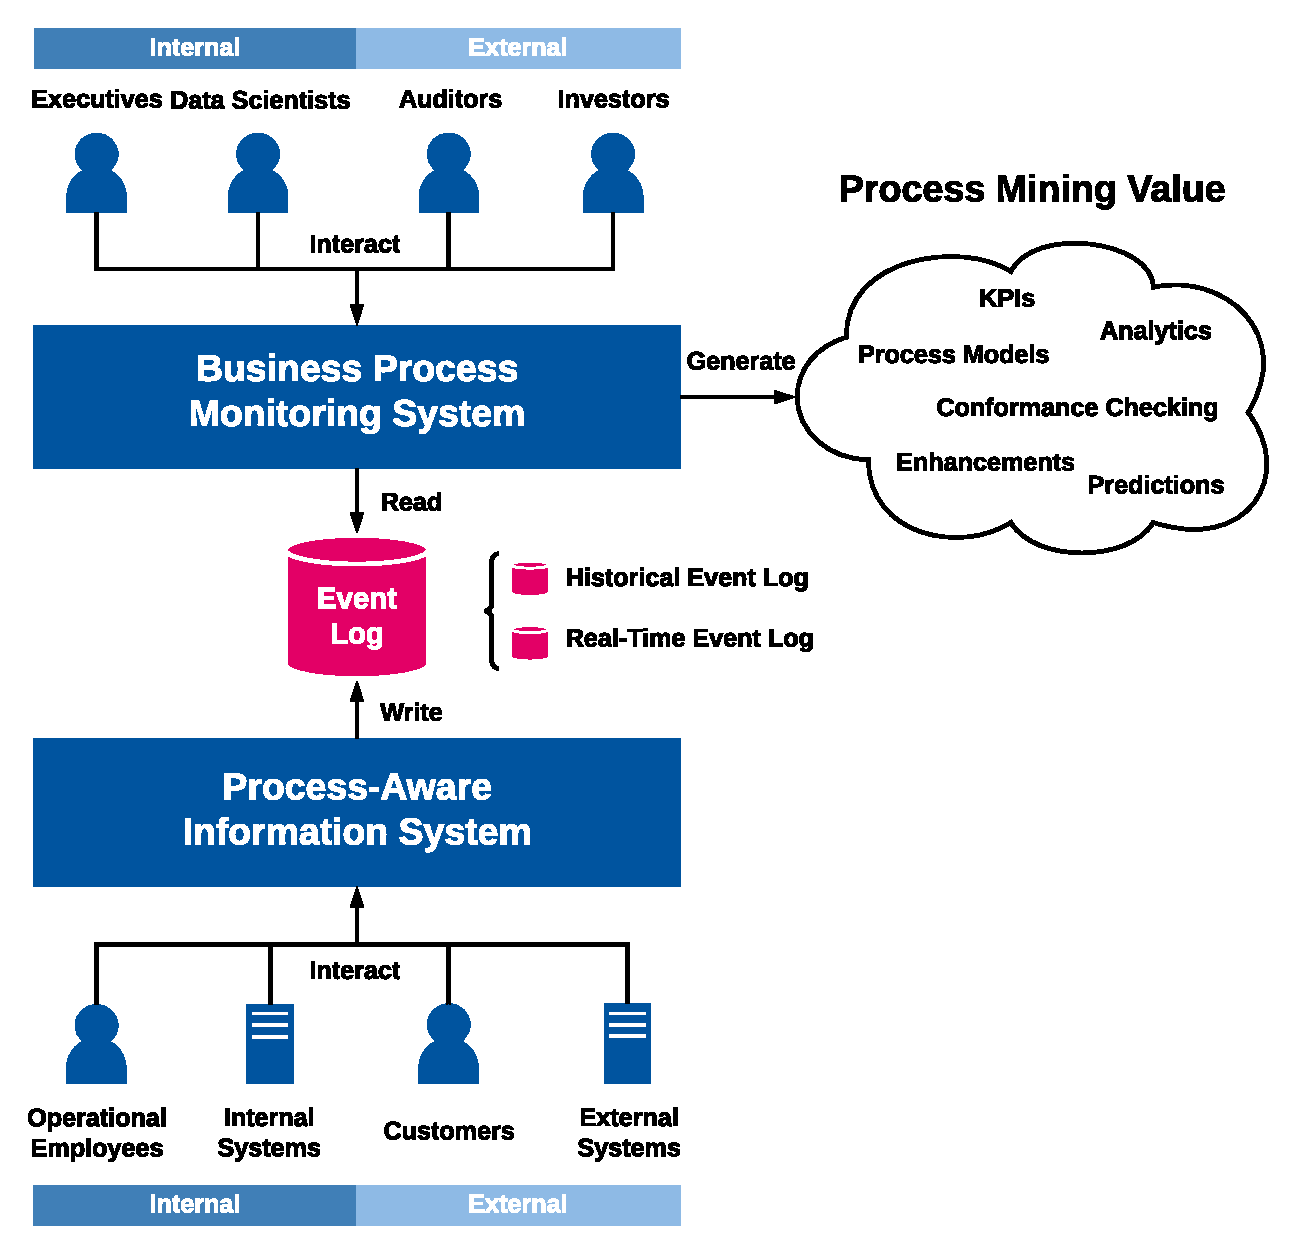
\includegraphics[width=\textwidth]{figures/process-monitoring}
	\caption[Process mining in the context of business process monitoring]{Business process monitoring allows to continuously apply process mining in an automated fashion in order to generate value for internal and external process stakeholders using the event data generated by a process-aware information system.}
	\label{fig:process-monitoring}
\end{figure}

Traditional process mining tends to be backward-looking \cite{DBLP:conf/scsc/Aalst18}, i.e. the main focus relies on analyzing and understanding past executions of a process rather than providing insights for running process instances in form of predictions or recommendations.
Businesses can develop a competitive advantage, if their process mining solution also offers predictive capabilities to anticipate the future of a running process instance.
For example, if it can be expected, that a running process instance will likely exceed its deadline, measures can be initiated before damage occurs.
Therefore, including the forward perspective is crucial for any competitive process mining software, especially in the context of business process monitoring.

\section{Problem Statement}

Although, many approaches for process prediction have been suggested in the literature (see Chapter \ref{chap:related_work}), current solutions are limited regarding the data they are able to consider and prediction task they can perform.
Many approaches derive their prediction purely from the control flow of a process instance ignoring additional data attributes in the event log.
Most notably, almost no approach is able to consider textual data for process prediction.
However, textual data is highly available in many systems and might hold important information, that can be used to improve the prediction performance.
In addition, most of the existing prediction methods focus on a single prediction task only, for example they just predict the remaining time or cycle time of a process instance.
Depending on the context, information about the next event or the future path of process instance can be of interest.
In some scenarios, processes instances have an outcome like success/failure or accepted/declined that can be predicted.

In data science, predictions are usually derived using \textit{predictive inference} \cite{predinf}, i.e. correlations in past observations are used to estimate target variables for new observations.
In the context of processes, past observations come in the form of historical event log data, that has been logged during the execution of a process.

This leads to the following problem statement:
Given an event log with past executions of a process holding numerical, categorical and textual data and a running (i.e. not completed) process instance, a prediction model is required that is able to reliably perform the following prediction tasks in order to answer the corresponding questions for a process owner:

\begin{itemize}
	\item Next activity prediction: What will happen next in the running process instance?
	\item Next event time prediction: When will the event happen?
	\item Case outcome prediction: What is the outcome of the process instance?
	\item Case cycle time prediction: When will the process instance finish?
	\item Future path prediction: What is the most likely future path of the process instance?
\end{itemize}

\begin{figure}[htbp!]
	\centering
	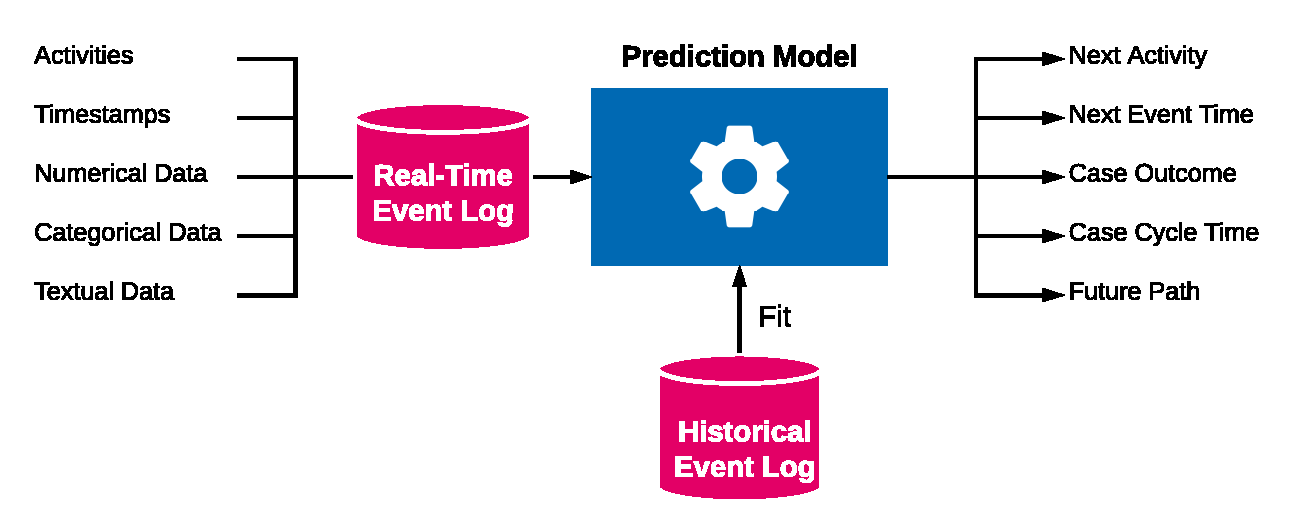
\includegraphics[width=\textwidth]{figures/problem-description}
	\caption[General process prediction model]{Predictive business process monitoring includes a prediction model, that is able to predict the future of running cases using historical event data. Current approaches differ in terms of the considered input data, the underlying prediction method and the prediction targets.}
	\label{fig:/problem-description}
\end{figure}

A general description of such a process prediction model is illustrated in Figure \ref{fig:/problem-description}.
Existing models follow the same framework, but they are less flexible in terms of input data types and prediction targets.
Including textual data for process prediction brings up new research questions, which are concretized in the next section.

\section{Research Goals and Questions}\label{sec:technology}

This thesis aims to improve current state-of-art approaches for process prediction in order to extend the capabilities of process monitoring software.
The main research goal is to design, implement and evaluate a predictive model for event data that is able to take advantage of additional textual data associated with each event in process.
Since most current approach are not able to handle textual data, the goal is to investigate if and to what extend textual data can improve the quality of process prediction.
Furthermore, different design choices and text models for text-aware process prediction need to be evaluated and potential trade-offs have to be discussed.
Finally, the text-aware process prediction model has to be compared to current state-of-the-art process prediction methods.

These goals lead to the formulation of the following three research questions:

\begin{enumerate}
	\item To what extend can the utilization of textual data improve the performance of process prediction?
	\item How does the choice of the text model and other parameters influence the prediction results?
	\item What are the advantages and disadvantages of the approach compared to existing methods?
\end{enumerate}



\section{Contribution}



\section{Thesis Structure}

This thesis is structured in seven chapters.
In Chapter \ref{chap:prelim} the basic notations, definitions and concepts used in this contribution are introduced.
This includes an brief introduction to process mining, text mining, supervised learning and LSTM neural networks.
Chapter \ref{chap:related_work} summarizes relevant scientific contributions, which focus on process prediction in process mining, and gives an overview of already available methods and their capabilities.
In Chapter \ref{chap:concept} a novel text-aware process prediction model as the main conceptional contribution is presented.
Moreover, Chapter \ref{chap:impl} covers the implementation details of the model on a technical level.
In Chapter \ref{chap:eval} the performance of the new approach is evaluated and compared to current state-of-the-art prediction methods.
Finally, the conclusion is given in Chapter \ref{chap:conclusion} by wrapping up the key achievements and discussing the limitations of the approach.
Furthermore, an outlook towards future potential research questions on process prediction in the context of business process monitoring is given.